\documentclass[12pt,a4paper]{article}

% ------------------------------------------------------------
% Configuración general
% ------------------------------------------------------------
\usepackage[utf8]{inputenc}
\usepackage[T1]{fontenc}
\usepackage[spanish,es-tabla]{babel}
\usepackage[a4paper,margin=2.5cm]{geometry}
\usepackage{setspace}
\setstretch{1.18}
\usepackage[sfdefault]{carlito}
\usepackage{graphicx}
\usepackage{float}
\usepackage{caption}
\usepackage{xcolor}
\usepackage{amsmath}
\usepackage{enumitem}
\usepackage{booktabs}
\usepackage{listings}
\usepackage{hyperref}

\hypersetup{
    colorlinks=true,
    linkcolor=blue!50!black,
    urlcolor=blue!50!black,
    citecolor=blue!50!black,
    pdftitle={Trabajo: Proyecciones 3D},
    pdfauthor={Sergio Andrés Majé Franco}
}

\definecolor{codebg}{RGB}{248,248,248}
\definecolor{codeframe}{RGB}{210,210,210}
\definecolor{codecomment}{RGB}{70,120,70}
\definecolor{codekeyword}{RGB}{40,70,150}

\lstdefinestyle{cstyle}{
    language=C,
    basicstyle=\ttfamily\footnotesize,
    keywordstyle=\color{codekeyword}\bfseries,
    commentstyle=\color{codecomment},
    numbers=left,
    numberstyle=\tiny\color{gray},
    numbersep=6pt,
    backgroundcolor=\color{codebg},
    frame=single,
    rulecolor=\color{codeframe},
    breaklines=true,
    tabsize=4,
    showstringspaces=false,
    captionpos=b
}

\setlist[itemize]{leftmargin=*, itemsep=0.2em, topsep=0.25em}
\setlist[enumerate]{leftmargin=*, itemsep=0.2em, topsep=0.25em}

\newcommand{\Universidad}{Universidad Internacional de La Rioja (UNIR)}
\newcommand{\Asignatura}{Informática Gráfica y Visualización}

\title{\textbf{Trabajo: Proyecciones 3D}\\Cuatro vistas de un mismo cubo en OpenGL}
\author{Sergio Andrés Majé Franco}
\date{\Asignatura \\ \Universidad \\ 28 de mayo de 2026}

\begin{document}

\maketitle
\tableofcontents
\newpage

\section{Introducción}

El presente documento describe la solución desarrollada para el trabajo \textit{Proyecciones 3D}. El informe se concentra en explicar la implementación realizada en OpenGL, presentar la captura del programa en ejecución y responder las preguntas solicitadas en la entrega. La redacción se mantiene enfocada en el resultado construido, sin extenderse hacia una investigación teórica externa al alcance de la actividad.

\section{Alcance de la entrega}

La actividad solicita una ventana OpenGL con cuatro vistas de un mismo cubo: proyección ortogonal, proyección gabinete, proyección perspectiva simétrica y proyección perspectiva oblicua. Además, el enunciado establece que la proyección debe realizarse sin mover el ojo desde la posición por defecto $(0,0,0)$, por lo que no se debe utilizar \texttt{gluLookAt()} ni una función equivalente de cámara.

La solución se entrega mediante un archivo \texttt{main.c}, en el que se implementa la ventana, la división en cuadrantes, las matrices de proyección y el dibujo de la escena. Este informe funciona como documento explicativo de la implementación y como evidencia visual del resultado obtenido.

\section{Descripción general de la solución}

El programa utiliza OpenGL clásico sobre X11/GLX. La ventana principal se divide en cuatro cuadrantes y cada cuadrante renderiza el mismo cubo con una configuración de proyección diferente. La geometría de la escena se mantiene común: un cubo con caras coloreadas, aristas resaltadas y ejes de referencia. Esta decisión permite que la comparación se centre en el efecto de las proyecciones y no en variaciones del objeto.

La estructura del código separa tres responsabilidades principales. Primero, se crea la ventana y el contexto gráfico. Luego, se definen funciones para construir matrices ortográficas, matrices de \emph{frustum} y una matriz de gabinete basada en cizalla. Finalmente, cada vista configura su propio \texttt{viewport}, carga su matriz de proyección y dibuja la escena común.

\begin{lstlisting}[style=cstyle,caption={Renderizado independiente de las cuatro vistas.},label={lst:render}]
configure_viewports(app, viewports);
glEnable(GL_SCISSOR_TEST);

drawOrthogonalView(&viewports[0]);
drawCabinetView(&viewports[1]);
drawSymmetricPerspectiveView(&viewports[2]);
drawObliquePerspectiveView(&viewports[3]);

draw_overlay(app, viewports);
\end{lstlisting}

El uso de funciones separadas facilita la revisión técnica, ya que cada proyección puede verificarse de manera aislada. También evita que la matriz de una vista afecte a las demás, debido a que cada cuadrante reinicia explícitamente las matrices de proyección y de modelo antes de dibujar.

\section{Implementación de las proyecciones}

\subsection{Proyección ortogonal}

La vista ortogonal se implementa mediante una matriz ortográfica. En esta proyección, los rayos proyectantes son paralelos y, por tanto, las aristas paralelas del cubo se conservan paralelas en la imagen final. Para que la figura sea más legible, el cubo se rota con una pose similar a una vista axonométrica, pero la proyección sigue siendo paralela y no genera puntos de fuga.

La matriz usada corresponde a la forma general de una proyección ortográfica:

\[
O =
\begin{bmatrix}
\frac{2}{r-l} & 0 & 0 & -\frac{r+l}{r-l} \\
0 & \frac{2}{t-b} & 0 & -\frac{t+b}{t-b} \\
0 & 0 & -\frac{2}{f-n} & -\frac{f+n}{f-n} \\
0 & 0 & 0 & 1
\end{bmatrix}
\]

\subsection{Proyección gabinete}

La proyección gabinete se desarrolló como una proyección oblicua paralela. La intención es conservar la cara frontal del cubo en verdadera magnitud o con una deformación mínima, mientras la profundidad se representa mediante una dirección diagonal reducida. Para lograrlo, se combina una proyección ortográfica con una matriz de cizalla sobre la profundidad.

La transformación conceptual aplicada es:

\[
    x' = x + k z \cos(\alpha), \qquad
    y' = y + k z \sin(\alpha)
\]

En la implementación se utiliza $k = 0.5$ y $\alpha = 45^\circ$. El valor $k=0.5$ corresponde a la reducción típica de una proyección gabinete, lo que evita que la profundidad se vea exagerada. Como el cubo se ubica delante del observador sobre valores negativos de $z$, el signo de la cizalla se ajusta para que la profundidad retroceda visualmente en diagonal.

\subsection{Perspectiva simétrica}

La perspectiva simétrica se implementa con una matriz de \emph{frustum} centrada. En esta vista se cumple que los límites laterales y verticales del volumen de visión son simétricos, es decir, $l=-r$ y $b=-t$. De esta manera, el volumen de proyección queda alineado con el eje de visión.

El cubo no se visualiza mediante movimiento de cámara. En cambio, se traslada como objeto hacia el eje $-Z$ para quedar dentro del volumen visible. Esta decisión respeta la restricción de mantener el ojo en $(0,0,0)$ y permite que la reducción por profundidad sea consecuencia de la matriz de perspectiva.

\subsection{Perspectiva oblicua}

La perspectiva oblicua se resolvió como una perspectiva \emph{off-axis}. A diferencia de la perspectiva simétrica, esta vista usa un \emph{frustum} asimétrico, con límites que no cumplen $l=-r$ o $b=-t$. El resultado es una perspectiva desplazada respecto al eje óptico, sin necesidad de mover el ojo ni de usar \texttt{gluLookAt()}.

La diferencia principal frente a la perspectiva simétrica está en la matriz de proyección, no en crear otro cubo ni en cambiar arbitrariamente la cámara. Por eso, el código conserva una colocación similar del objeto en ambas vistas de perspectiva y hace que el contraste dependa del volumen de visión.

\begin{lstlisting}[style=cstyle,caption={Diferencia entre frustum simétrico y frustum asimétrico.},label={lst:frustum}]
/* Perspectiva simetrica: frustum centrado */
build_frustum_matrix(-right, right, -top, top, 3.0, 24.0, projection);

/* Perspectiva oblicua: frustum asimetrico u off-axis */
build_frustum_matrix(-1.65 * right, 0.35 * right,
                     -1.05 * top, 0.95 * top,
                     3.0, 24.0, projection);
\end{lstlisting}

\section{Evidencia de ejecución}

\begin{figure}[H]
    \centering
    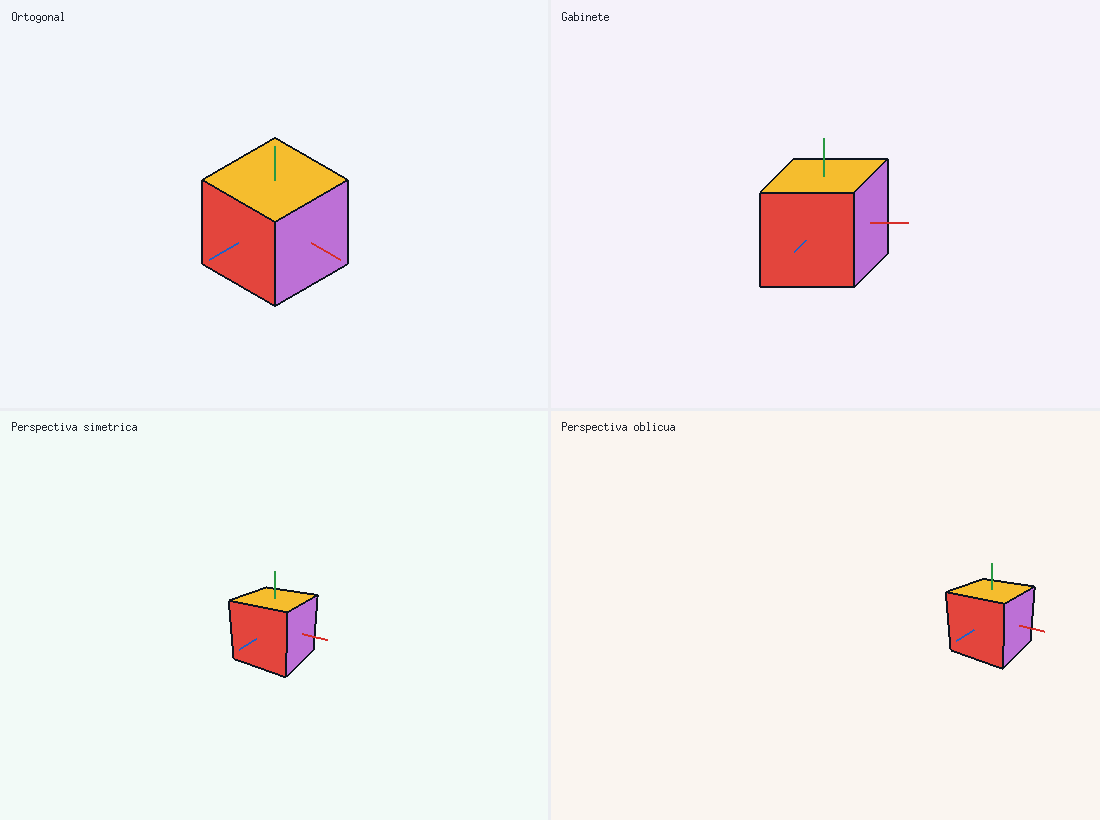
\includegraphics[width=0.96\textwidth]{../captures/proyecciones-3d-review-final.png}
    \caption{Ventana principal del programa con cuatro vistas del mismo cubo.}
    \label{fig:proyecciones}
\end{figure}

La Figura~\ref{fig:proyecciones} muestra la ventana principal del programa. En el cuadrante superior izquierdo se observa la proyección ortogonal; en el superior derecho, la proyección gabinete; en el inferior izquierdo, la perspectiva simétrica; y en el inferior derecho, la perspectiva oblicua. Las etiquetas permiten identificar cada caso y los colores del cubo ayudan a comparar el comportamiento espacial de las caras en las cuatro vistas.

La vista ortogonal conserva el paralelismo de las aristas. La gabinete mantiene una cara frontal dominante y desplaza la profundidad en diagonal. La perspectiva simétrica muestra una proyección centrada, mientras que la perspectiva oblicua desplaza el volumen visible mediante un \emph{frustum} asimétrico. Aunque las dos perspectivas conservan una pose cercana del cubo, su diferencia se encuentra en la configuración del volumen de proyección.

\section{Visualización complementaria: hiperboloide de una hoja}

Además de la ventana principal con las cuatro proyecciones del cubo, se documenta una visualización complementaria desarrollada dentro del laboratorio. Esta sección tiene como finalidad dejar evidencia de la aplicación de OpenGL en una geometría tridimensional más compleja que un sólido básico, reutilizando la lógica de ejes, representación espacial y construcción gráfica de una escena 3D.

La superficie representada corresponde a un hiperboloide de una hoja definido por la ecuación:

\[
    \frac{x^2}{4} + \frac{(y-3)^2}{9} - \frac{(z+1)^2}{16} = 1
\]

Esta expresión describe una superficie cuadrática centrada en $(0,3,-1)$. Para su visualización se emplea una representación alámbrica, ya que la malla permite observar la continuidad de la superficie y su curvatura sin ocultar la estructura geométrica. En términos prácticos, este tipo de representación es útil para comprobar cómo una parametrización matemática puede transformarse en coordenadas renderizables dentro de una escena OpenGL.

Una forma conveniente de generar la superficie consiste en parametrizarla mediante funciones hiperbólicas:

\[
    x = 2\cosh(v)\cos(u), \qquad
    y = 3 + 3\cosh(v)\sin(u), \qquad
    z = -1 + 4\sinh(v)
\]

con $u$ recorriendo el ángulo alrededor del eje de la superficie y $v$ controlando la apertura de la malla. Al acotar el intervalo de $v$, se obtiene una porción visible y manejable de la superficie, evitando que la figura crezca de forma excesiva dentro de la ventana.

\begin{figure}[H]
    \centering
    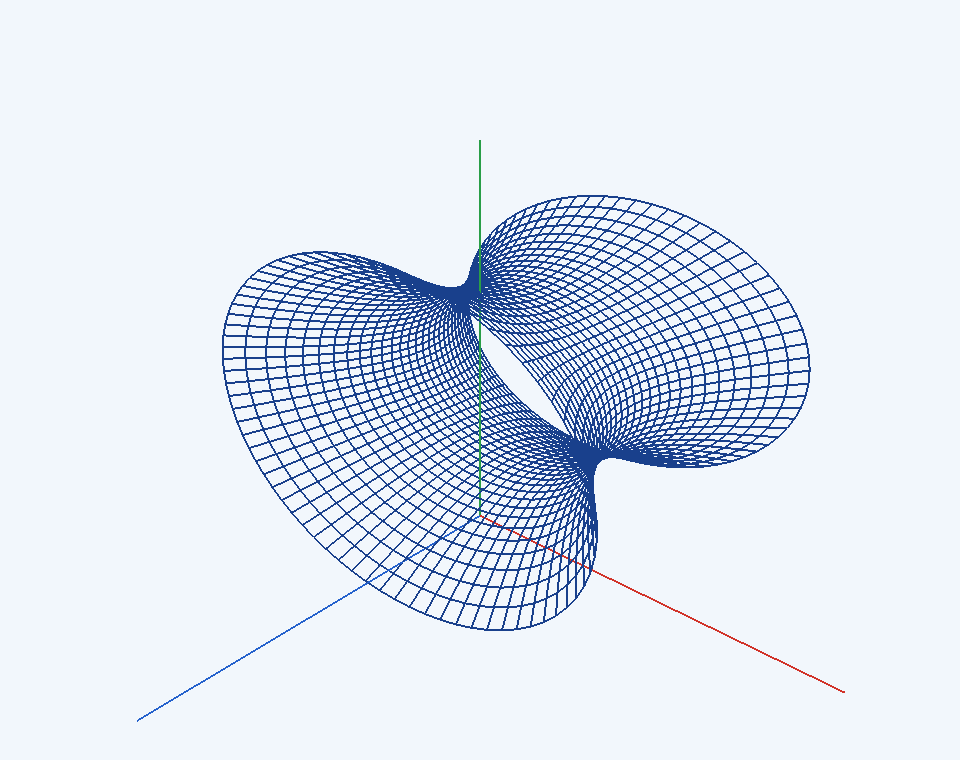
\includegraphics[width=0.82\textwidth]{../../../extras/calculo-vectorial-figura-1/captures/figura1.png}
    \caption{Representación alámbrica de un hiperboloide de una hoja en OpenGL.}
    \label{fig:hiperboloide}
\end{figure}

La Figura~\ref{fig:hiperboloide} complementa la entrega al mostrar que el laboratorio no se limita al cubo empleado para comparar proyecciones, sino que también permite representar superficies matemáticas mediante mallas paramétricas. Esta sección refuerza la relación entre geometría, cálculo vectorial y visualización computacional, que es uno de los aspectos prácticos de la informática gráfica.


\section{Verificación de requisitos}

\begin{table}[H]
\centering
\caption{Relación entre el requisito de la actividad y la solución implementada.}
\label{tab:requisitos}
\begin{tabular}{p{0.36\textwidth}p{0.52\textwidth}}
\toprule
\textbf{Requisito} & \textbf{Cumplimiento} \\
\midrule
Ventana con cuatro vistas & La ventana se divide en cuatro cuadrantes mediante \texttt{glViewport()} y \texttt{glScissor()}. \\
Mismo cubo en todas las vistas & La escena se dibuja desde una función común que reutiliza el cubo, las aristas y los ejes. \\
Proyección ortogonal & Se usa una matriz ortográfica y una pose axonométrica del objeto. \\
Proyección gabinete & Se combina una matriz ortográfica con una cizalla de profundidad reducida. \\
Perspectiva simétrica & Se usa un \emph{frustum} centrado con límites simétricos. \\
Perspectiva oblicua & Se usa un \emph{frustum} asimétrico para obtener una perspectiva \emph{off-axis}. \\
No mover el ojo & No se usa \texttt{gluLookAt()}; el objeto se traslada hacia $-Z$ dentro de la escena. \\
Archivo principal único & La implementación se concentra en \texttt{main.c}. \\
\bottomrule
\end{tabular}
\end{table}

\section{Funcionamiento del programa}

\subsection{¿Funciona bien el programa?}

Sí. El programa cumple el objetivo de la actividad, porque abre una única ventana OpenGL y muestra cuatro vistas simultáneas del mismo cubo. Cada cuadrante tiene una etiqueta propia y aplica una configuración de proyección distinta. Además, la solución evita el uso de \texttt{gluLookAt()} y mantiene el ojo en la posición por defecto, usando transformaciones del objeto y matrices de proyección para construir la escena.

Desde el resultado visual, la vista ortogonal es la más directa de validar porque mantiene las aristas paralelas. La vista gabinete representa la profundidad mediante una cizalla oblicua con reducción. La perspectiva simétrica se apoya en un \emph{frustum} centrado, y la perspectiva oblicua se diferencia mediante un \emph{frustum} asimétrico. En conjunto, el programa permite comparar las cuatro formas de proyección solicitadas sobre una misma geometría.

\subsection{¿Qué fallos existen?}

No se identifican fallos funcionales que impidan cumplir la actividad. Sin embargo, se reconocen algunas limitaciones propias de la implementación:

\begin{itemize}
    \item El programa depende de un entorno compatible con X11/GLX y OpenGL clásico, por lo que su ejecución directa está orientada a sistemas que soporten ese entorno gráfico.
    \item Las etiquetas se dibujan con una fuente bitmap sencilla mediante \texttt{glXUseXFont}; es suficiente para la práctica, pero no busca una presentación tipográfica avanzada.
    \item Los parámetros de escala, traslación y amplitud del \emph{frustum} fueron ajustados manualmente para priorizar que las cuatro vistas se observaran completas y centradas.
    \item La diferencia entre la perspectiva simétrica y la perspectiva oblicua es moderada para no recortar el cubo dentro del cuadrante. Puede exagerarse aumentando la asimetría del \emph{frustum}, aunque eso reduciría la estabilidad visual de la captura.
\end{itemize}

Estas limitaciones no contradicen el enunciado. Más bien, delimitan el alcance de una solución académica enfocada en demostrar las cuatro proyecciones solicitadas de forma clara y ejecutable.

\section{Conclusiones}

El informe permite evidenciar que la solución desarrollada responde al alcance solicitado: una ventana OpenGL con cuatro vistas de un mismo cubo y con proyecciones diferenciadas. La explicación se centró en el documento, en la captura de ejecución y en las decisiones técnicas principales necesarias para justificar el resultado.

La implementación es defendible porque separa la escena común de las matrices de proyección. Esta separación evita interpretar las cuatro vistas como simples rotaciones del cubo y permite explicar por qué cada cuadrante corresponde a una proyección distinta. La restricción sobre la cámara también se cumple, ya que no se mueve el ojo desde $(0,0,0)$ ni se utiliza \texttt{gluLookAt()}.

En términos de entrega, el programa funciona correctamente para el objetivo planteado. Las limitaciones identificadas se relacionan con el entorno gráfico, la sencillez del rotulado y el ajuste manual de parámetros visuales, pero no afectan el cumplimiento central de la actividad.

La visualización del hiperboloide complementa el documento porque amplía la evidencia práctica del laboratorio hacia la representación de superficies paramétricas. Con ello se muestra que la implementación no solo permite comparar proyecciones sobre un cubo, sino también trasladar conceptos matemáticos a una escena 3D renderizada con OpenGL.

\section{Archivos adjuntos}

Junto con este informe se adjunta un archivo comprimido con el código fuente completo de la solución, incluyendo el archivo \texttt{main.c}. Además, se anexa el enlace al repositorio de GitHub que contiene el laboratorio:

\begin{center}
\href{https://github.com/smaje99/computer-graphics-and-visualization-unir}{https://github.com/smaje99/computer-graphics-and-visualization-unir}
\end{center}

\end{document}
